\documentclass[../jarvis.tex]{subfiles}
\graphicspath{{\subfix{../images/}}}
\usepackage{scrambledenvs}
\newscrambledenv{hint}
\begin{document}
Trigonometric identities are \textit{triggier} than you may realise! However, they are also useful in many ways, from parametrisations to geometry, and even bridging over to complex numbers.
\begin{figure}[H]
    \centering
    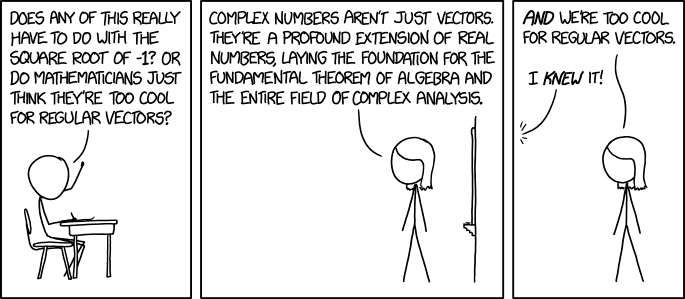
\includegraphics[scale=0.5]{xkcd_complex_numbers.png}
    \caption{Comic from https://xkcd.wtf/2028/}
\end{figure}

\begin{proposition}[Trigonometric Identities]
    Let $A$ and $B$ denote angles.
    \begin{enumerate}
        \item \textit{Pythagorean Identity}: $\sin^2A+\cos^2A=1$
        \begin{enumerate}
            \item $\tan^2A+1=\sec^2A$,
            \item $\cot^2A+1=\csc^2A$.
        \end{enumerate}
        \item Addition Formulae
        \begin{enumerate}
            \item $\sin(A\pm B)=\sin A\cos B\pm \cos A\sin B$,
            \item $\cos(A\pm B)=\cos A\cos B\mp \sin A\sin B$,
            \item $\tan(A\pm B)=\frac{\tan A\pm\tan B}{1\mp \tan A\tan B}.$
        \end{enumerate}
        \item Double Angle Formulae
        \begin{enumerate}
            \item $\sin 2A=2\sin A\cos A$,
            \item $\cos 2A=\cos^2A-\sin^2A=2\cos^2A-1=1-2\sin^2A,$
            \item $\tan 2A=\frac{2\tan A}{1-\tan^2 A}.$
        \end{enumerate}  
        \item Sum-to-Product Formulae
        \begin{enumerate}
            \item $\sin A+\sin B=2\sin\left(\frac{A+B}{2}\right)\cos\left(\frac{A-B}{2}\right),$
            \item $\sin A-\sin B=2\cos\left(\frac{A+B}{2}\right)\sin\left(\frac{A-B}{2}\right),$
            \item $\cos A+\cos B=2\cos\left(\frac{A+B}{2}\right)\cos\left(\frac{A-B}{2}\right),$
            \item $\cos A-\cos B=-2\sin\left(\frac{A+B}{2}\right)\sin\left(\frac{A-B}{2}\right).$
        \end{enumerate}
    \end{enumerate}
\end{proposition}
\begin{proposition}[Trigonometric R Method (or R-formula)]
    Let $a,b,\theta$ be reals. The R-formula expresses the \textit{weighted sum} $a\sin\theta+b\cos\theta$ as a single $\sin$ or $\cos$ term.

    Letting $R=\sqrt{a^2+b^2}$ and $\tan\alpha=\frac{b}{a}$,
    \begin{enumerate}
        \item \textit{Sine form:} $a\sin\theta\pm b\cos\theta=R\sin(\theta\pm\alpha).$
        \item \textit{Cosine form:} $a\cos\theta\pm b\sin\theta=R\cos(\theta\mp\alpha).$
    \end{enumerate}
\end{proposition}
\section{Applying Identities \ez}
For fundamentals, it is important that we are able to simplify complicated expressions into simpler forms.
\begin{example}
    Simplify $\cos{49^{\dg}}+\cos{71^{\dg}}$ as a single trigonometric term.
\end{example}
\begin{proof}
    Observe the symmetry about $60$: $49=60-11$ and $71=60+11$, so
    \begin{align*}
        \cos{49^{\dg}}+\cos{71^{\dg}}&=\cos{(60-11)^{\dg}}+\cos{(60+11)^{\dg}} \\
        &=2\cos{60^{\dg}}\cos{11^{\dg}} \\
        &=\boxed{\cos{11^{\dg}}}.
    \end{align*}
\end{proof}

\begin{proposition}[Toolkit]
    There usually isn't much to do with trigonometry. Most useful properties relate the sum or difference of angles, and so the usual techniques go by:
    \begin{enumerate}
        \item squaring and adding the given relations,
        \item squaring and subtracting the given relations,
        \item simply adding or subtracting the given relations,
        \item multiplying the given relations, 
        \item using sum-to-product formulae, or
        \item expressing the required expression in terms of the given angles.
    \end{enumerate}
\end{proposition}

\begin{example}[2020 SMO(S) P9]
If $8\cos{x}-8\sin{x}=3$, find the value of $\tan{x}+\frac{1}{\tan{x}}$.
\end{example}
\begin{proof}
    Firstly, $(8\cos{x}-8\sin{x})^2=64-64\sin{2x}=9 \implies \sin{2x}=\frac{55}{64}$.
    
    Moreover, $$\tan{x}+\frac{1}{\tan{x}}=\frac{\sin{x}}{\cos{x}}+\frac{\cos{x}}{\sin{x}}=\frac{2}{\sin{2x}}=\boxed{\frac{128}{55}}.$$
\end{proof}

\begin{example}[2021 SMO(O) P1]
    It is given that $\frac{\pi}{2}<\beta<\alpha<\frac{3\pi}{4}$, $\cos{(\alpha-\beta)}=\frac{12}{13}$ and $\sin{(\alpha+\beta)}=-\frac{3}{5}$. Find $\floor{|2021\sin{2\alpha}|}$.
\end{example}
\begin{proof}
    From the angle conditions, we have $0<\alpha-\beta<\frac{\pi}{4}$ and $\pi<\alpha+\beta<\frac{3\pi}{2}$. We now pull a big sneaky! Note that 
    \begin{align*}
        \sin{2\alpha}&=\sin{((\alpha-\beta)+(\alpha+\beta))} \\
        &=\sin{(\alpha-\beta)}\cos{(\alpha+\beta)}+\cos{(\alpha-\beta)}\sin{(\alpha+\beta)} \\
        &=\frac{5}{13}\cdot\left(-\frac{4}{5}\right)+\frac{12}{13}\cdot\left(-\frac{3}{5}\right) \\
        &=-\frac{4}{13}-\frac{36}{65} \\
        &=-\frac{56}{65}.
    \end{align*}
    Thus, $$\floor{|2021\sin{2\alpha}|}=\floor{\frac{2021\cdot56}{65}}=\floor{\frac{113176}{65}}=\boxed{1741}.$$
\end{proof}


\begin{example}[2021 SMO(O) P12]
    Given that $\sin{\alpha}+\sin{\beta}=\frac{1}{10}$ and $\cos{\alpha}+\cos{\beta}=\frac{1}{9}$. Find the value of $\floor{\tan^2(\alpha+\beta)}$.
\end{example}
\begin{proof}
    By the sum-to-product formulae,
    $$\frac{\sin{\alpha}+\sin{\beta}}{\cos{\alpha}+\cos{\beta}}=\tan{\left(\frac{A+B}{2}\right)}=\frac{9}{10}.$$

    Thus,
    \begin{align*}
        \floor{\tan^2{(\alpha+\beta)}}&=\floor{\left(\frac{2\tan{\left(\frac{A+B}{2}\right)}}{1-\tan^2{\left(\frac{A+B}{2}\right)}}\right)^2}\\
        &=\floor{\left(\frac{2\cdot\frac{9}{10}}{1-\frac{81}{100}}\right)^2}\\
        &=\floor{\left(\frac{180}{19}\right)^2}=\floor{\frac{32400}{361}} \\
        &=\boxed{89}.
    \end{align*}
\end{proof}

\begin{example}[2021 SMO(S) P7]
    If $\cos{A}-\cos{B}=\frac{1}{2}$ and $\sin{A}-\sin{B}=-\frac{1}{4}$, find the value of $100\sin{(A+B)}.$
\end{example}
\begin{proof}
    With some foresight, we notice that squaring and then summing or subtracting the relations wouldn't be too useful at this point.

    We turn to the sum-to-product formulae:
    \begin{equation}\label{trig-p7-1}
        \cos{A}-\cos{B}=\frac{1}{2} \implies \sin{\frac{A+B}{2}}\sin{\frac{A-B}{2}}=-\frac{1}{4},
    \end{equation}
    and 
    \begin{equation}\label{trig-p7-2}
        \sin{A}-\sin{B}=-\frac{1}{4} \implies \cos{\frac{A+B}{2}}\sin{\frac{A-B}{2}}=-\frac{1}{8}.
    \end{equation}

    Now, squaring seems like a good idea:
    $$\eqref{trig-p7-1}^2+\eqref{trig-p7-2}^2=\sin^2{\frac{A-B}{2}=\frac{5}{64}}.$$
    Moreover, 
    $$\eqref{trig-p7-1}\cdot\eqref{trig-p7-2}=\frac{1}{2}\sin{A+B}\sin{\frac{A-B}{2}}=\frac{1}{32}.$$
    Thus, $100\sin(A+B)=100\cdot\frac{4}{5}=80.$
\end{proof}

\begin{example}[2018 SMO(S) P17]
    Let 
    $$L=\sum_{k=7}^{16}\left(1+\tan(15k^{\dg}+15^{\dg})\tan15k^{\dg}\right).$$
    Find $\floor{L}$.
\end{example}
\begin{proof}
    We see that the expression is dominated by tangents, and that the summand resembles the denominator of the tangent addition formula!

    For simplicity, let $A=15k^{\dg}+15^{\dg}$ and $B=15k^{\dg}$, then $L=\sum_{k=7}^{16}\left(1+\tan{A}\tan{B}\right).$

    To simplify this sum, consider 
    \begin{align*}
        L\cdot\tan(A-B)&=L\cdot\tan 15^{\dg}\\
        &=\sum_{k=7}^{16}\tan{(A-B)}\left(1+\tan{A}\tan{B}\right) \\
        &=\sum_{k=7}^{16} \left(\tan{A}-\tan{B}\right)=\sum_{k=7}^{16} \left(\tan{\left(15k^{\dg}+15^{\dg}\right)}-\tan{15k^{\dg}}\right)\\
        &=\left(\tan{120^{\dg}}-\tan{105^{\dg}}\right)+\left(\tan{135^{\dg}}-\tan{120^{\dg}}\right)+\cdots+\left(\tan{255^{\dg}}-\tan{240^{\dg}}\right) \\
        &=\tan{255^{\dg}}-\tan{105^{\dg}} \\
        &=2\tan{75^{\dg}}
    \end{align*}
    To this end, we first compute $\tan{15^{\dg}}$:
    $$\tan{30^{\dg}}=\frac{\sqrt{3}}{3}=\frac{2\tan{15^{\dg}}}{1-\tan^2{15^{\dg}}} \implies \tan{15^{\dg}}=2-\sqrt{3}.$$
    Then, 
    \begin{align*}
        L&=\frac{2\tan{75^{\dg}}}{\tan{15^{\dg}}}=\frac{2\tan{(30+45)^{\dg}}}{2-\sqrt{3}} \\
        &=\frac{4+2\sqrt{3}}{2-\sqrt{3}}\cdot\frac{2+\sqrt{3}}{2+\sqrt{3}}\\
        &=14+8\sqrt{3}.
    \end{align*}
    Finally, since $1.7<\sqrt{3}<1.75$,
    $$14+8\cdot1.7=27.6 < L=14+8\sqrt{3} < 14+8\cdot1.75=28,$$
    thus $\floor{L}=\boxed{27}$.
\end{proof}

\begin{example}[2021 SMO(S) P15]
    Find the minimum value of $$\frac{8}{\sin{2\theta}}+12\tan{\theta},$$
    where $0<\theta<\frac{\pi}{2}.$
\end{example}
\begin{proof}
    \begin{align*}
        \frac{8}{\sin{2\theta}}+12\tan{\theta}&=\frac{4+12\sin^2{\theta}}{\sin{\theta}\cos{\theta}} \\
        &=\frac{16\sin^2{\theta}+4\cos^2{\theta}}{\sin{\theta}\cos{\theta}} \\
        &\geq \frac{2\sqrt{64\sin^2{\theta}\cos^2{\theta}}}{\sin{\theta}\cos{\theta}} \quad\text{by AM-GM}\\
        &=\boxed{16}.
    \end{align*}
    Equality occurs when $4\cos^2{\theta}=16\sin^2{\theta} \implies \tan{\theta}=\frac{1}{2}$, for which $\theta$ lies in the given domain.
\end{proof}

\subsection{Sums and Products \ez}
As a disclaimer, some parts of this section may tie into complex numbers, so you may wish to omit these parts until you have had some form of treatment on the connection between complex numbers and trigonometry.

That said, most of this section should be self-contained, and we do our best to not tie into complex numbers, although sometimes they may be used as motivation. This is just a testament to the interconnectedness between these two beautiful ideas!

\begin{example}[2014 SMO(S) P33]
    Find the value of $$2\tan{1^{\dg}}(\sin{2^{\dg}}+\sin{4^{\dg}}+\cdots+\sin{178^{\dg}}).$$    
\end{example}
With some foresight, we first note the useful identity that \begin{equation}\label{trig-p33-1}
    \cos{A-1}+\cos{A+1}=2\cos{A}\cos{1}
\end{equation}
\begin{proof}
    Let $S=\sin{2^{\dg}}+\sin{4^{\dg}}+\cdots+\sin{178^{\dg}}$,
    then 
    \begin{align*}
        S&=2(\sin{2^{\dg}}+\sin{4^{\dg}}+\cdots+\sin{178^{\dg}}+\sin{180^{\dg}}) \\
        &=2(\sin{2^{\dg}}+\sin{4^{\dg}}+\cdots+\sin{88^{\dg}})+1\\
        &=2(\cos{2^{\dg}}+\cdots)+(\cos{0^{\dg}}+\cos{90^{\dg}})\\
        &=(\cos{0^{\dg}}+\cos{2^{\dg}})+(\cos{2^{\dg}}+\cos{4^{\dg}})+\cdots+(\cos{88^{\dg}}+\cos{90^{\dg}})\\
        &=2\cos{1^{\dg}}(\cos{1^{\dg}}+\cos{3^{\dg}}+\cdots+\cos{89^{\dg}}) \quad\text{using \eqref{trig-p33-1}}\\
    \end{align*}
    Now, we use a trick to simplify the terms:
    \begin{align*}
        S&=\cot{1^{\dg}}(2\sin{1^{\dg}}\cos{1^{\dg}}+2\sin{3^{\dg}\cos{1}+\cdots+2\sin{89^{\dg}}}\cos{1}) \\
        &=\cot{1^{\dg}}((\sin{2^{\dg}}-\sin{0^{\dg}})+(\sin{4^{\dg}-\sin{2^{\dg}}})+\cdots+(\sin{90^{\dg}}-\sin{88^{\dg}}))\\
        &=\cot{1^{\dg}}(\sin{90^{\dg}}-\sin{0^{\dg}})=\cot{1^{\dg}}.
    \end{align*}
    Hence, the required value is $\boxed{2}$.
\end{proof}
\begin{example}[2013 AIME I/14]
    For $\pi\leq\theta\leq2\pi,$ let
    $$P=\frac{1}{2}\cos{\theta}-\frac{1}{4}\sin{2\theta}-\frac{1}{8}\cos{3\theta}+\frac{1}{16}\sin{4\theta}+\frac{1}{32}\cos{5\theta}-\frac{1}{64}\sin{6\theta}-\frac{1}{128}\cos{7\theta}+\cdots$$
    and
    $$Q=1-\frac{1}{2}\sin{\theta}-\frac{1}{4}\cos{2\theta}+\frac{1}{8}\sin{3\theta}+\frac{1}{16}\cos{4\theta}-\frac{1}{32}\sin{5\theta}-\frac{1}{64}\cos{6\theta}+\frac{1}{128}\sin{7\theta}+\cdots$$
    so that $\frac{P}{Q}=\frac{2\sqrt{2}}{7}.$ Find the value of $\sin{\theta}$.
\end{example}
Surely $P$ and $Q$ are connected by some obscure relation - this is almost by design! For the confused reader (I sure was!) who can't spot the pattern just yet, the terms in $P$ and $Q$ have signs that oscillate in the pattern of $(+,-,-,+)$, while the trigonometric terms oscillate between $\sin$ and $\cos$.

The terms in $P$ and $Q$ are quite unruly, so let us attempt to line them up. A naive attempt would be to first "unify" the $\cos{\theta}$ term from $P$ and the $\sin{\theta}$ term from $Q$ by considering $P\cdot\sin{\theta}$ and $Q\cdot\cos{\theta}$.

Now, for each term in $P$ and $Q$ with the same coefficient, note that we have the identities
$$\begin{cases}
    \sin{n\theta}\cos{\theta}+\cos{n\theta}\sin{\theta}=\sin{(n+1)\theta} \\
    \cos{n\theta}\sin{\theta}-\sin{n\theta}\cos{\theta}=\cos{(n+1)\theta}.
\end{cases}$$
Somehow, we now have the miraculous identity:
$$P\cdot\sin{\theta}-Q\cdot\cos{\theta}=-2P.$$

Dividing across by $Q$ yields $$\frac{P}{Q}=\frac{\cos{\theta}}{\sin{\theta}+2}=\frac{2\sqrt{2}}{7},$$
and squaring and simplifying produces the quadratic
$$57\sin^2{\theta}+32\sin{\theta}-17=0 \implies (19\sin{\theta}+17)(3\sin{\theta}-1)=0.$$
Since $\pi\leq\theta\leq2\pi$, $\sin{\theta}<0$ so $\sin{\theta}=\boxed{-\frac{17}{19}}$ only.
\section{Some Geometry}
As it turns out, many concepts of a triangle is unified through its \textit{area}.

We start by asserting (without proof) the sine and cosine law. Let $A,B,C$ be angles in a triangle and let $a,b,c$ be the lengths opposite their respective angles.

\begin{proposition}[Sine Law]
    Given a triangle $ABC$,
    $$\frac{a}{\sin{A}}=\frac{b}{\sin{B}}=\frac{c}{\sin{C}}.$$
\end{proposition}
\begin{proposition}[Cosine Law]
    Given a triangle $ABC$,
    $$c^2=a^2+b^2-2ab\cos{C}$$.
    Upon a rearrangement, we also have the useful form
    $$\cos{C}=\frac{a^2+b^2-c^2}{2ab}.$$
\end{proposition}
\subsection{Lengths \ez}
Trigonometry is very closely related to the (unit) circle. We have seen the sine rule, but as it turns out, the sine rule can also tie in neatly to the circumcircle. This is the so-called \textit{extended} sine rule:
\begin{proposition}[Extended sine rule]
    $$\frac{a}{\sin{A}}=\frac{b}{\sin{B}}=\frac{c}{\sin{C}}=2R$$
\end{proposition}
It suffices to show that $\frac{a}{\sin{A}}=2R$, and certainly, $2R$ is the diameter of the circumcircle. It would thus make sense to tie in its diameter.
\begin{figure}[H]
    \centering
    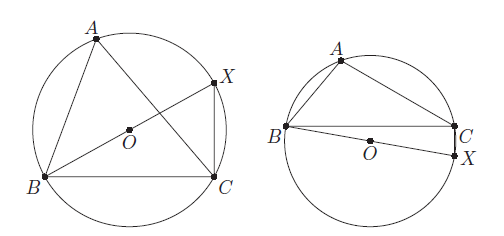
\includegraphics[scale=1]{egmo_extended_LOS.PNG}
    \caption{Two setups of the Sine Rule. \protect\footnotemark}
\end{figure}
\footnote{From Euclidean Geometry in Mathematical Olympiads by Evan Chen, pp.52.}

\begin{proof}
    Let $BX$ be a diameter of the circumcircle as above. Then, $BXC$ is a right triangle with right angle at $C$. Thus, $BC=a$, $BX=2R$. Moreover, either $\angle BXC=\angle BAC$ or $\angle BXC=\pi-\angle BAC$.
    
    In any case, $\sin{A}=\sin{\angle BXC}=\frac{a}{2R}$, and we are done.
\end{proof}

We have seen setups involving a circle and a triangle, but what about a circle and \textit{two} triangles?

A canonical result is \textbf{Ptolemy's theorem}.
\begin{theorem}[Ptolemy's Theorem]
    Let $ABCD$ be a cyclic quadrilateral. Then,
    $$AB\cdot CD+AD\cdot BC=AC\cdot BD.$$
\end{theorem}
There are certainly more elegant proofs involving similar triangles, complex numbers, \textit{inversion}, etc. But here, we showcase a trigonometric approach.

We should first anticipate what our mode of attack should look like. While this is a result involving lengths, it is obstructive to work purely in lengths since we don't have a way to tie in to the cyclic nature of the setup.

On the other hand, angles should work nicely because angles uniquely define our quadrilateral.
\begin{remark}
    This may be counterintuitive, since this is a length result! However this should be expected: we don't really care about each individual length, but rather \textit{how} each length relates to each other.
\end{remark} 
\begin{figure}[H]
    \centering
    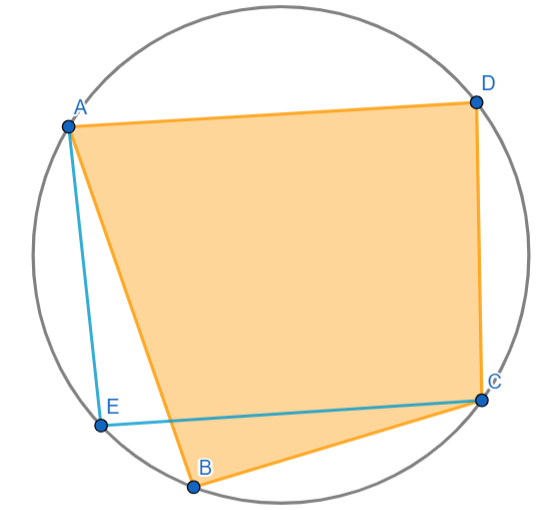
\includegraphics[scale=0.8]{ptolemy.PNG}
    \caption{Looks kind of neat to be honest.}
\end{figure}
With some foreshadowing, we consider the area of our quadrilateral $ABCD$, as well as the area of another useful quadrilateral. Ideally, we want our second quadrilateral to have an easily computable area. 
\begin{proof}
    Let $E$ be the point such that $BE$ is parallel to $AC$.
    
    Then,
    \begin{align*}
        [ABCD]&=[ADE]+[DCE] \\
        &=\frac{1}{2}\left(AD\cdot AE\sin{\angle DAE}+CD\cdot CE\sin{\angle DCE}\right) \\
        &=\frac{1}{2}\left(AD\cdot AE+CD\cdot CE\right)\sin{\angle DAE} \\
    \end{align*}
    where the third equality follows since $\sin{\angle DAE}=\sin{\angle DCE}$ and the last equality follows because $AEBC$ is an isosceles trapezium.
    
    On the other hand, if we let $X$ be the intersection of the diagonals $AC$ and $BD$, then 
    \begin{align*}
        [ABCD]&=\frac{1}{2}\cdot AC\cdot BD \sin{\angle BXC} \\
        &=\frac{1}{2}\cdot AC\cdot BD\sin{\angle XBE}= \frac{1}{2}\cdot AC\cdot BD\sin{\angle DBE} \\
        &=\frac{1}{2}\cdot AC\cdot BD\sin{\angle DCE}=\frac{1}{2}\cdot AC\cdot BD\sin{\angle DAE}.
    \end{align*}
    Thus, \begin{align*}
        &\frac{1}{2}\left(AD\cdot AE+CD\cdot CE\right)\sin{\angle DAE}=\frac{1}{2}\cdot AC\cdot BD\sin{\angle DAE} \\
        &\implies AB\cdot CD+AD\cdot BC=AC\cdot BD.
    \end{align*}
\end{proof}

An immediate-ish consequence of Ptolemy's theorem is Stewart's theorem, which allows us to find the length of a \textit{cevian}.

\begin{theorem}[Stewart's Theorem]
    Let $ABC$ be a triangle and let $D$ be a point on $BC$. Define also $m=DB, n=DC, d=AD$. Then
    $$man+ad^2=b^2m+c^2n.$$
\end{theorem}
This is also written in the more comical form
$$man+dad=bmb+cnc,$$ which fits into a nifty mnemonic
"a \textit{man} and his \textit{dad} put a \textit{bomb} in the \textit{sink}."

We present two proofs - the first is a consequence of Ptolemy's theorem.

\begin{figure}[H]
    \centering
    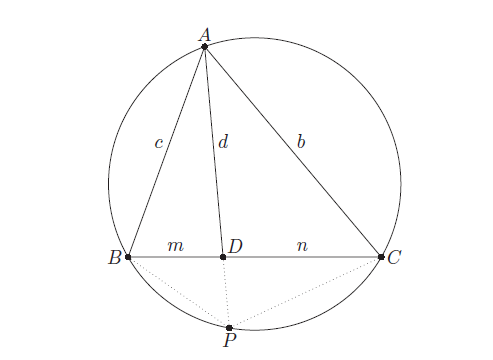
\includegraphics[scale=0.8]{egmo_stewart.PNG}
    \caption{$AD$ is a cevian of $ABC$.}
\end{figure}

\begin{proof}
    Let the ray $AD$ meet the circumcircle of $ABC$ again at $P$. Then, $BDP \sim ADC$ and $CDP\sim ADB$, whence
    $$\frac{BP}{b}=\frac{m}{d}\quad\text{and}\quad \frac{CP}{c}=\frac{n}{d}.$$
    Moreover, by \textit{power of a point},
    $$DP=\frac{mn}{d}.$$
    
    Finally, by Ptolemy's theorem,
    \begin{align*}
        AP\cdot BC&=AC\cdot BP+AB\cdot CP \\
        a\left(d+\frac{mn}{d}\right)&=b\cdot\frac{bm}{d}+c\cdot\frac{cn}{d} \\
        ad^2+man&=b^2m+c^2n.
    \end{align*}
\end{proof}

Our second proof goes by way of applying the cosine rule to point $D$ in two ways.
\begin{proof}
    $$\frac{n^2+d^2-b^2}{2dn}=\cos{\angle ADC}=-\cos{\angle ADB}=-\frac{d^2+m^2-c^2}{2dm}.$$
    This gives
    $$n(d^2+m^2-c^2)+m(n^2+d^2-b^2)=0,$$
    upon which expanding and simplifying gives the result.
\end{proof}

\subsection{Area Results \ez}
With these results, it turns out that we can formulate the area of a triangle in many different ways. For convenience, we denote the area of a triangle $ABC$ as $[ABC]$.
\begin{theorem}[Area of a Triangle]
    \begin{align*}
        [ABC] &=\frac{1}{2}ab\sin{C}=\frac{1}{2}bc\sin{A}=\frac{1}{2}ca\sin{B} \\
        &=\sqrt{s(s-a)(s-b)(s-c)} \\
        &=rs.
    \end{align*}
    Here, $r$ is the \textbf{inradius} and $s=\frac{1}{2}(a+b+c)$ is the \textbf{semiperimeter} of $ABC$.
\end{theorem}
The relation $[ABC]=\sqrt{s(s-a)(s-b)(s-c)}$ is the so-called \textbf{Heron's formula}, and allows us to relate the side lengths of a triangle to it's semiperimeter and inradius.

To prove this, we consider the \textbf{contact triangle} of $ABC$. The contact triangle is the triangle formed from the three points of tangency of the incircle.
\begin{figure}[H]
    \centering
    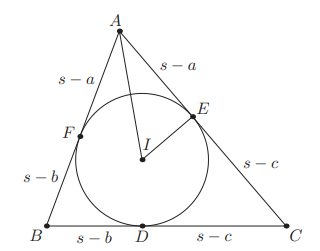
\includegraphics[scale=1]{egmo_herons_contact.PNG}
    \caption{$DEF$ is the contact triangle of $ABC$.\protect\footnotemark}
\end{figure}
\footnote{From Euclidean Geometry in Mathematical Olympiads by Evan Chen, pp.78.}
We state, again without proof, the key trigonometric identity of use here:
\begin{lemma}
    If $A,B,C$ are angles in a triangle and are each acute, then 
    $$\tan{A}+\tan{B}+\tan{C}=\tan{A}\tan{B}\tan{C}.$$
\end{lemma}
The proof of this is sneakily left as a problem in the exercises section.

\begin{proof}
    Now, we have
    $$\tan{\frac{\pi}{2}-\frac{A}{2}}=\tan{\angle AIF}=\frac{s-a}{r},$$
    and similarly,
    $$\tan{\frac{\pi}{2}-\frac{B}{2}}=\tan{\angle BID}=\frac{s-b}{r}$$
    $$\tan{\frac{\pi}{2}-\frac{C}{2}}=\tan{\angle CIE}=\frac{s-c}{r}.$$
    
    Since we have $\left(\frac{\pi}{2}-\frac{A}{2}\right)+\frac{\pi}{2}-\frac{A}{2}+\frac{\pi}{2}-\frac{A}{2}=\pi$,
    our lemma gives, helpfully,
    \begin{align*}
        \frac{s-a}{r}+\frac{s-b}{r}+\frac{s-c}{r}&=\frac{s-a}{r}\cdot\frac{s-b}{r}\cdot\frac{s-c}{r} \\
        &=\frac{3s-(a+b+c)}{r} \\
        &=\frac{s}{r}.
    \end{align*}
    Finally, $(sr)^2=s(s-a)(s-b)(s-c)$, as needed.
\end{proof}
\section{Parametrising \med}
Consider the unit circle $x^2+y^2=1$. Then, we may describe the set of points along the circumference of the circle as
$$(x,y)=(\cos\theta, \sin\theta), \quad -\pi\leq\theta\leq\pi.$$
We say that this is a \textit{parametrisation} of the set of points on the circle.

And certainly, the circle $x^2+y^2=r^2$ with radius $r$ is simply a scaled unit circle, so it's points can be described as
$$(x,y)=(r\cos\theta, r\sin\theta), \quad -\pi\leq\theta\leq\pi.$$

This idea is extremely useful to re-parametrise conditions and to maximise or minimise the so-called objective functions.
\begin{example}[2018 SMO(S) P11]
    Let $x$ and $y$ be real numbers. Find the maximum value of $2x^2-3xy-2y^2$ subject to the condition that
    $$25x^2-20xy+40y^2=36.$$
\end{example}
The "cross-term" $20xy$ suggests that we should complete the square. 

\begin{proof}
    Write $$25x^2-20xy+40y^2=(25x^2-20xy+4y^2)+36y^2=(5x-2y)^2+36y^2=36.$$
    
    Now, let $36a^2=(5x-2y)^2$, then $36a^2+36y^2=36 \implies a^2+y^2=1$, and so we may parametrise 
    $$(a,y)=(\cos\theta,\sin\theta),\quad -\pi\leq\theta\leq\pi \implies (x,y)=\left(\frac{6\cos\theta+2\sin\theta}{5}, \sin\theta\right).$$
    
    Thus, \begin{align*}
        2x^2-3xy-2y^2&=\frac{2(6\cos\theta+2\sin\theta)^2-15(6\cos\theta+2\sin\theta)\sin\theta-50\sin^2\theta}{25} \\
        &=\frac{2(36\cos^2\theta+12\sin 2\theta+4\sin^2\theta)-(45\sin2\theta+30\sin^2\theta)-50\sin^2\theta}{25} \\
        &=\frac{72\cos^2\theta-72\sin^2\theta-21\sin2\theta}{25} \\
        &=\frac{72\cos2\theta-21\sin2\theta}{25} \\
        &=\frac{\sqrt{72^2+21^2}\cos(2\theta+\alpha)}{25}, \quad \text{where }\tan\alpha=\frac{21}{72} \\
        &\geq\frac{\sqrt{72^2+21^2}}{25}=\boxed{3}.
    \end{align*}
    
    The minimum occurs when $2\theta=-\tan^{-1}\frac{21}{72}$, which lies in the domain of $\theta$.
\end{proof}

\section{Exercises}
\subsection{Warmup}
\problem Let $ABC$ be a triangle. Prove that 
\begin{enumerate}
    \item $[ABC]=\frac{abc}{4R}$,
    \begin{hints}
        \begin{hint}
            Sine rule.
        \end{hint}
    \end{hints} 
    \item $[ABC]=rs$.
    \begin{hints}
        \begin{hint}
            Draw a good diagram.
        \end{hint}
        \begin{hint}
            Divide $[ABC]$ into the area of three right triangles.
        \end{hint}
    \end{hints}
\end{enumerate}
\problem If $A,B,C$ are angles in a triangle and are each acute, prove that $$\tan{A}+\tan{B}+\tan{C}=\tan{A}\tan{B}\tan{C}.$$
\begin{hints}
    \begin{hint}
        $C=\pi-(A+B)$.
    \end{hint}
\end{hints}

\problem[Parallelogram Law]Let $ABCD$ be a parallelogram. Prove that the sum of the lengths of the squares of four sides of $ABCD$ equals the sum of the squares of the length of its two diagonals.

In other words, prove that
$$2(AB^2+BC^2)=AC^2+BD^2.$$
\begin{hints}
    \begin{hint}
        Apply the cosine rule to triangles $BAD$ and $ADC$.
    \end{hint}
\end{hints}
\problem[Apollonius's Theorem]Let $ABC$ be a triangle and let $M$ be the midpoint of $BC$. Prove that 
$$AB^2+AC^2=2(AM^2+\left(\frac{BC}{2}\right)^2).$$
\begin{hints}
    \begin{hint}
        Extend $AM$ to a point $N$ so that $AM=MN$. Can you apply the parallelogram law?
    \end{hint}
\end{hints}
\problem[Angle Bisector Theorem]Let $ABC$ be a triangle and let $D$ be a point on $BC$ such that $AD$ bisects $\angle BAC$. Prove that $$\frac{BD}{CD}=\frac{AB}{AC}.$$
\begin{hints}
    \begin{hint}
        Apply the sine rule to triangles $ABD$ and $ACD$.
    \end{hint}
\end{hints}
\problem[Tangent Rule] Let $A,B,C$ be angles in a triangle and let $a,b,c$ denote the side length of the triangle opposite each respective angle. Prove that
$$\frac{a-b}{a+b}=\frac{\tan{\frac{A+B}{2}}}{\tan{\frac{A-B}{2}}}.$$
\begin{hints}
    \begin{hint}
        Prove that $\frac{a-b}{a+b}=\frac{\sin{A}-\sin{B}}{\sin{A}+\sin{B}}.$
    \end{hint}
    \begin{hint}
        Use the sum-to-product identities.
    \end{hint}
\end{hints}
\problem[Catastrophic Cancellation] Let $A,B,C$ be angles in a triangle and let $a,b,c$ denote the side length of the triangle opposite each respective angle.

Using the tangent rule, prove that $$\tan{\frac{A-B}{2}}=\frac{a-b}{a+b}\cot{\frac{C}{2}}.$$

\begin{enumerate}
    \item In the time before digital calculators, the tangent rule is preferred over the cosine rule when used to find a missing length when given two side lengths $a,b$ and their enclosed angle $C$. Why is this so?
    \item For small values of $C$, is the tangent rule still preferred?
\end{enumerate}

\problem[Cotangent rule] Let $A,B,C$ be angles in a triangle and let $a,b,c$ denote the side length of the triangle opposite each respective angle. Prove that 
$$\frac{\cot{\frac{A}{2}}}{s-a}=\frac{\cot{\frac{B}{2}}}{s-b}=\frac{\cot{\frac{C}{2}}}{s-c}=\frac{1}{r}.$$
\begin{hints}
    \begin{hint}
        Find an expression for $\cot{\frac{A}{2}}.$
    \end{hint}
    \begin{hint}
        Consider the triple cotangent identity.
    \end{hint}
\end{hints}

\problem[Mollweide's Formulas] Prove that
\begin{enumerate}
    \item $$\frac{a+b}{c}=\frac{\cos{\frac{A-B}{2}}}{\sin{\frac{C}{2}}}.$$
    \begin{hints}
        \begin{hint}
            Start from $\frac{\cos{\frac{A}{2}-\frac{B}{2}}}{\cos{\frac{A}{2}}+\cos{\frac{B}{2}}}.$
        \end{hint}
        \begin{hint}
            Convert everything to cotangents. You may also need to use the second problem. 
        \end{hint}
    \end{hints}
    \item $$\frac{a-b}{c}=\frac{\sin{\frac{A-B}{2}}}{\cos{\frac{C}{2}}}.$$
    \begin{hints}
        \begin{hint}
            $\cos{\frac{C}{2}}=\sin{\frac{A}{2}+\frac{B}{2}}$.
        \end{hint}
        \begin{hint}
            Convert everything to cotangents.
        \end{hint}
    \end{hints}
\end{enumerate}

\subsection{Problems}
\problem[2017 SMO(O) P13]Let $ABC$ be a triangle with $\angle A=30^{\circ}$. If $b^2=a^2+bc$, find $\angle C$.
\begin{hints}
    \begin{hint}
        Use cosine rule.
    \end{hint}
\end{hints}

\problem[2019 SMO(O) P18] In triangle $ABC$, $BC=10$, $CA=9$, $\cos{C}=\frac{5}{14}$. The angle bisector of $C$ meets the circumcircle again at $N$, the altitude from $A$ meets the circumcircle again at $L$ and $NL$ intersects $BC$ at $M$. Find the length of $MC$.
\begin{hints}
    \begin{hint}
        Draw $LB$.
    \end{hint}
    \begin{hint}
        Use the angle bisector theorem on $BLD$.
    \end{hint}
    \begin{hint}
        Find $CD$.
    \end{hint}
\end{hints} 
\problem[2021 SMO(O) P8] Find the minimum value of $(x+7)^2+(x+4)^2$ subject to the constraint $(x-5)^2+(y-7)^2=4$.
\begin{hints}
    \begin{hint}
        Parametrise $x$ and $y$ in terms of sines and cosines.
    \end{hint}
\end{hints}
\problem[2021 SMO(O) P18] Let $ABC$ be a triangle with $AB=10$ and
$$\frac{\cos{A}}{\cos{B}}=\frac{b}{a}=\frac{4}{3}.$$
Let $P$ be a point on the incircle of $ABC$. Find the maximum value of $$PA^2+PB^2+PC^2.$$
\begin{hints}
    \begin{hint}
        Prove that $ABC$ is a right-angled triangle.
    \end{hint}
    \begin{hint}
        You may find it convenient to impose the setup on the cartesian plane. Let $C=(0,0)$ and define $A,B$ in a similar way.
    \end{hint}
    \begin{hint}
        Find the inradius of the incircle and hence parametrise $P$ in terms of sines and cosines.
    \end{hint}
\end{hints}
\problem[2016 SMO(O) P23]Let $ABC$ be an acute-angled triangle with circumcenter $O$. Suppose $AC=92$, $\tan{\angle OAB}=\frac{1}{7}$ and $\angle CAO=3\angle OAB$. Find the length of $AB$.
\begin{hints}
    \begin{hint}
        Find $\tan{\angle CAO}$.
    \end{hint}
\end{hints}
\problem[2022 AIME I/15] Let $x,y,z$ be positive reals satisfying the following system of equations:
\begin{align*}
    \sqrt{2x-xy}+\sqrt{2y-xy}&=1 \\
    \sqrt{2y-yz}+\sqrt{2z-yz}&=\sqrt{2} \\
    \sqrt{2z-zx}+\sqrt{2x-zx}&=\sqrt{3}.
\end{align*}
Find the value of $[(1-x)(1-y)(1-z)]^2.$\begin{hints}
    \begin{hint}
        What is the domain of $x,y,z$?
    \end{hint}
    \begin{hint}
        Let $x=2\sin^2{\theta}$. Why can we do this?
    \end{hint}
\end{hints}

\subsection{Challenges}
\problem[2017 SMO(O) P25]In a triangle $ABC$, $AB=AC$, $BC=22\sqrt{3}$ and $\cos{A}=-\frac{17}{225}$. Let $D$ be a point on $AC$ such that $AD<DC$ and $P$ be the point on the segment $BD$ such that $\angle APC=90^{\circ}$. Given that $\angle ABD=\angle BCP$, find the length of $BD$.

\problem[2021 Taiwan APMO Preliminary I]In triangle $ABC$, $\angle A=23^{\circ}$ and $\angle B=46^{\circ}$. Let $\Gamma$ be a circle with center $C$ with radius $AC$ and let the angle bisector of $B$ intersect $\Gamma$ at $M$ and at $N$. Find $\angle MAN$.
\begin{hints}
    \begin{hint}
        Let $D$ be the foot of perpendicular from C onto the angle bisector of $B$ and let $C'$ be the foot of perpendicular from C onto $BC$.
    \end{hint}
    \begin{hint}
        Use the extended sine law to find $MN$. You may also note that $MN=2MC'$.
    \end{hint}
    \begin{hint}
        Use the law of sines to find $\frac{BC}{AC}$.
    \end{hint}
\end{hints}
\problem[2019 SMO(O) P15] In triangle $ABC$, $AB=209$, $BC=171$, $CA=190$ and $M$ is the midpoint of $BC$. Point $L$ lies on the extension of $BA$ and point $N$ lies on the extension of $MA$ such that points $C,L,N$ are collinear and $AL=NL$. Find the length of $AN$.
\begin{hints}
    \begin{hint}
        Construct a point $K$ such that $ABKC$ is a parallelogram.
    \end{hint}
    \begin{hint}
        Use Apollonius' theorem on a convenient triangle.
    \end{hint}
    \begin{hint}
        Find $NK$.
    \end{hint}
\end{hints}
\problem[2019 SMO(O) P17] Two circles are tangent to each other internally at point $T$. Let chord $AB$ of the larger circle be tangent to the smaller circle at $P$. If $AB=\frac{59}{\sqrt{3}}$, $TA=32$ and $TB=27$, find the length of $TP$.
\begin{hints}
    \begin{hint}
        Prove that $TP$ bisects $\angle ATB$. This is called the death star lemma or the shooting lemma (This is a useful lemma, so google a proof if you have to!).
    \end{hint}
    \begin{hint}
        Stewart's Theorem.
    \end{hint}
\end{hints}
\section{Hints}
\printhint
\section{Solutions to Selected Problems}
\paragraph{2017 SMO(O) P13} By cosine rule, 
$$a^2=b^2+c^2-2bc\cos{A}=b^2+c^2-\sqrt{3}bc.$$
Given that $b^2=a^2+bc$, we have
\begin{align*}
    a^2=a^2+bc+c^2-\sqrt{3}bc &\iff c^2+bc=\sqrt{3}bc \\
    &\iff c=(\sqrt{3}-1)b. 
\end{align*}
This also gives $$a^2=(2-\sqrt{3})b^2 \implies a=\sqrt{2-\sqrt{3}}b=\sqrt{\left(\frac{\sqrt{3}-1}{2}\right)^2}b=\frac{\sqrt{3}-1}{\sqrt{2}}b.$$

Hence, \begin{align*}
    \cos{C}&=\frac{a^2+b^2-c^2}{2ab} \\
        &=\frac{(2-\sqrt{3})+1-(4-2\sqrt{3})}{\sqrt{2}(\sqrt{3}-1)} \\
        &=\frac{\sqrt{3}-1}{\sqrt{2}(\sqrt{3}-1)}=\frac{1}{\sqrt{2}}.
\end{align*}
Thus, $\angle C=\boxed{45^{\circ}}$.

\paragraph{2017 SMO(O) P25}
Now, we look for a way to tie in the two conditions, with the goal of eventually tying down $AD$:
\begin{enumerate}
    \item $\angle DPC=90^{\circ}$, and
    \item $\angle ABD=\angle BCP$.
\end{enumerate}
This motivates us to draw the circumcircle of $APC$ and hence let $M$ be the circumcenter of $APC$. Then, $M$ is the midpoint of $AC$ since $APC$ is right-angled, implying $AC$ is the diameter. This then gives the convenient lengths:
$$AM=MC=PM.$$

We also have the angles $$\angle MCP=\angle MPC\quad\text{and}\quad \angle ABD=\angle BCP.$$
Noting that $ABC$ is isosceles with $AB=BC$, it follows that $\angle CBP=\angle MCP=\angle MPC$, and that $\angle DPM=\angle ABD=\angle BCP$. Now, by sine rule on $ABD$ and $PDM$, we have
$$\frac{AD}{AB}=\frac{\sin{\angle ABD}}{\sin{\angle ADB}}$$
and 
$$\frac{DM}{PM}=\frac{\sin{\angle DPM}}{\sin{\angle PDM}}=\frac{\sin{\angle DPM}}{\sin{\angle ADB}}=\frac{AD}{AB}.$$

We now return to focus on $AD$:
$$\frac{AD}{AC}=\frac{AD}{AB}=\frac{DM}{PM}=\frac{AM-AD}{MC}=\frac{AC-2AD}{AC},$$
whence $AC=3AD$.

Finally, by cosine rule on $ABC$ and $ABD$, $BD^2=\boxed{28}.$
\end{document}